\documentclass[]{article}
\usepackage{todonotes}
\usepackage[T1]{fontenc}
\usepackage{lmodern}
\usepackage{amssymb,amsmath}
\usepackage{ifxetex,ifluatex}
\usepackage{fixltx2e} % provides \textsubscript
\usepackage[utf8]{inputenc}
\usepackage{color}
\usepackage[unicode=true]{hyperref}
\hypersetup{breaklinks=true,
            bookmarks=true,
            pdfauthor={Patrik Jansson et al.},
            pdftitle={GRACeFUL D4.2: A Domain Specific Language (DSL) for GRACeFUL Concept Maps},
            colorlinks=true,
            citecolor=blue,
            urlcolor=blue,
            linkcolor=magenta,
            pdfborder={0 0 0}}
\urlstyle{same}  % don't use monospace font for urls
\setlength{\parindent}{0pt}
\setlength{\parskip}{4pt plus 2pt minus 1pt}
\setlength{\emergencystretch}{3em}  % prevent overfull lines

%% Cezar
\usepackage[margin=1.60in]{geometry}
\usepackage[verbose]{wrapfig}
\usepackage{graphicx}
\usepackage{subfig}
\usepackage{rotating}
\usepackage{lscape}
\usepackage{float}
\usepackage{geometry}
\usepackage{framed}
\definecolor{GRACeFULblue}{rgb}{0.20,0.60,0.86}

\author{}
\date{}

\begin{document}

\begin{center}

\includegraphics[width=5cm]{../coverpage/GRACeFULlogo.png}

\textcolor{GRACeFULblue}{Global systems Rapid Assessment tools\\
through Constraint FUnctional Languages}

\vspace{1cm}

FETPROACT-1-2014 Grant Nº 640954

\end{center}

\begin{framed}
\begin{center}
\Large
A Domain Specific Language (DSL) for \\
GRACeFUL Concept Maps\\[1ex]

D4.2\\[1ex]

\end{center}
\end{framed}

\vspace{1cm}

\noindent
\begin{tabular}{@{}ll@{}}
  Lead Participant:       & Chalmers (M. Algehed, S. Einarsdóttir, A. Gerdes, and P. Jansson)
\\Partners Contributing:  & KU Leuven, UPC
\\Dissemination Level:    & PU
\\Document Version:       & Draft (version 2017-01-19)
\\Date of Submission:     & 2017-01-31
\\Due Date of Delivery:   & 2017-01-31
\end{tabular}

\newpage

\section*{A Domain Specific Language (DSL) for\\GRACeFUL Concept Maps}\label{DSL4GRACeFUL}

\vfill

\tableofcontents

\vfill

\newpage

\section*{Abstract}\label{abstract}

This second deliverable of WP4 includes a short overview of a Domain
Specific Language (DSL) for description of GRACeFUL concept maps, and
a formal semantics in terms of types and functions. This is a
continuation of the initial work described in ``D4.1 Formal Concept
Maps Elements Descriptions'' delivered in project month 6. The actual
source code implementing the DSL is freely available in the project
repository on GitHub: \url{https://github.com/GRACeFUL-project/}.

\section{Introduction}\label{introduction}

% explain what we mean with an GCM, restricted version: semi-qualitative version
% of CLDs

% Use a DSL as a kind of intermediate representation

% Not easy to translate from a visual diagram directly to CP

% Overview of Graceful, at least the bit of our concern, place the DSL in context

This document reports on second deliverable (D4.2) of work package 4 of the
\grace project. The main task of this work package is to build a \emph{\ac{DSL}}
for \acp{GCM}. A \ac{GCM} is a representation of policy analysis that contains
all the elements of a policy problem definition, such as goals, criteria, and
a description of the system. A \ac{GCM} is developed and manipulated by
stakeholders during \ac{GMB} sessions. Ultimately a \ac{GCM} is translated
(via the \ac{DSL}) to a \ac{CFP}, which is analysed by a constraint solver. The
results of the constraint solver are presented to the stakeholders.

The \ac{DSL} can be regarded as an intermediate layer between the visual
representation of a \acf{GCM} and a corresponding constraint program.
Translating the visual representation directly to a constraint program is
difficult, because it is hard to check if the generated program is correct. A
DSL alleviates this problem and us to validate the correctness of a model. In
addition, a \ac{DSL} improves the scalability by abstracting away from the
constraint solver. In the longer term this will lead to a \ac{DSL} aimed at
building scalable \acp{RAT} for collective policy making in Global Systems.  

% How have the definitions from D4.1 changed

In the previous deliverable~\cite{d4.1} we have formalised the various elements
of \acp{GCM}. Progressive insight learned us that \acp{CLD} are not
adequate to model the systems the project is envisioning, such as for the \ac{CRUD}
case study. Instead of using \aclp{CLD} we now use
\emph{stock-and-flow} diagram to model the system dynamics. Stock-and-flow
diagrams allow for a more detailed (semi-)quantative analysis.

% We have constructed a DSL, link to github

We have implemented the \acl{DSL} in the functional programming language
Haskell~\cite{haskell98}. Haskell is the so-called host language in which the
\ac{DSL} is embedded. Language features such as algebraic datatypes,
higher-order functions, lazy evaluation, and a rich type system makes Haskell
particulary suitable for defined \acp{DSL}. The details of this language are
explained in Section~\ref{sec:gl}. The actual source code implementing the DSL
is freely available in the project repository on
GitHub\footnote{\url{https://github.com/GRACeFUL-project/}}.

% Explain the structure of the rest of the doc

We continue this document by giving the necessary background information, in
Section~\ref{sec:background}, for making the remaining sections more accessible.
We present the details of the \ac{DSL} for \acp{GCM} including some examples in
Section~\ref{sec:gl}. Finally, we give the formal semantics of the \ac{DSL} in
Section~\ref{sec:semantics}.


\section{Background}

\todo{write a short background about some of these concepts}

DSL?

Semi-qualitative modelling

Constraint programming

Factors, Criteria, Actions

Outcomes: help the stakeholders

\begin{itemize}
\item find alternative policies that can satisfy the goals,
\item identify inconsistencies in the problem definition,
\item  present visualisations of possible future trajectories.
\end{itemize}

The information from and for the stakeholders will go through at least
two layers of the GRACeFUL system before it reaches the constraint
solver. First, through the graphical visual interface, which will
assist the stakeholders in building the problem definition, and which
will present the results of the qualitative simulations, and second,
the DSLs which will translate between these interfaces and the
constraint programming layer.

GRACeFUL concept maps

TODO: use part of the commented text:

% The description of the system is elicited from stakeholders
% with help from the GRACeFUL system, which contains a library of relevant
% factors, relating them to the concepts under discussion. Here, the term
% \emph{factors} refers to \emph{characteristics of a system that can take
% a value, either quantitative or qualitative, that can change over time}
% (source: the \emph{GRACeFUL Glossary of Terms}). In mathematical system
% theory, a collection of factors correspond to the \emph{state} of the
% system. Similarly, \emph{external factors} correspond to \emph{inputs}
% to the system. As such, factors are assumed to be associated with
% measurable (if only in qualitative terms) values.
%
% As in systems theory, a distinction is made between inputs that are
% beyond the control of the system, and which are potentially uncertain
% (or even unknown), and \emph{actions} or combinations of actions, which
% represent the system theoretical \emph{controls}, generally assumed to
% be deterministic but with uncertain consequences.
%
% The interaction between the factors, and between the factors and the
% criteria, represents a first description of the system (no alternatives
% are present, or only the baseline policy is assumed to be active). This
% description is in the form of a \emph{causal loop diagram}. A causal
% loop diagram is a form of \emph{directed, simple, labelled graph}, i.e.:
%
% \begin{enumerate}
% \def\labelenumi{\alph{enumi}.}
% \item
%   a link between two nodes has a well-defined source and a target (it is
%   \emph{directed}); intuitively, the link represents a causal relation
%   between the source (cause) and the target (effect);
% \item
%   there can be at most one connection from one node to another (the
%   graph is \emph{simple}): either a causal relation exists, or it does
%   not. Note, however, that since the graph is directed, there may be an
%   inverse connection from the ``effect'' to the ``cause'', as in
%   feedback loops;
% \item
%   the connections are either \emph{positive} (an increase in the value
%   of the source causes an increase in the value of the target), or
%   \emph{negative} (an increase causes a decrease), hence the graph is
%   \emph{labelled}.
% \end{enumerate}
%
% It can be seen from the last point that nodes \emph{must} represent
% values that can be partially ordered. This rules out nodes that
% represent, say, stakeholders.
%
% As an example, two such causal loop diagrams, produced in the
% student sessions organised as part of the CRUD case study, can be
% found in the Appendix.
%
% The GRACeFUL system can assist in building the causal loop diagram, for
% example by suggesting connections, or by pointing out inconsistencies.
%
% At this stage, if we can attribute qualitative values to the various
% nodes, the causal loop diagram describes a system that can make the
% object of a qualitative simulation. The criteria play the roles of
% constraints: the qualitative trajectories that lead outside the criteria
% can be pruned by the constraint programming system.
%
% The causal loop diagram is enhanced to a GRACeFUL concept map by the
% addition of extra nodes and non-causal links. The extra nodes represent
% actions, goals, alternatives, and stakeholders.
%
% Like all previous elements, the actions are also obtained from the
% stakeholders. As explained in the previous section, actions are the
% components of alternatives, among which will be found the policy
% solutions we are seeking. Alternatives are, according to the GRACeFUL
% Glossary of Terms, ``action or combination of actions that influence the
% values of criteria''. They correspond to Walker's ``alternative
% policies'', where a \emph{policy} is defined ``loosely'' as ``a set of
% actions taken to solve a problem''. As in the case of goal definition,
% the GRACeFUL system can suggest such ``atomic actions'' that are useful
% to the goals in the context of the problem at hand.
%
% The role of actions in the GRACeFUL concept maps is to give initial
% values to the factors and criteria they influence. They do not link via
% causal loops to these factors, since actions are not of the requisite
% type (they do not represent values that can increase or decrease).
% However, they will usually have non-causal links, representing
% constraining relationships to the factors.
%
% In the other cases of extra nodes (goals, alternatives, and
% stakeholders), the links represent primarily ``belongs to''
% relationships: there are links from stakeholders to goals, indicating
% which stakeholders have declared which goals; there are links from goals
% to the criteria by which they are assessed; finally, there are links
% between alternatives and the factors and criteria that they (i.e., their
% constituent atomic actions) influence.
%
% Figure \ref{fig:cm} (drawn by Sadie McEvoy (Deltares)) shows a
% graphical representation of the structure of a GRACeFUL concept map:
%
% \begin{figure}[!ht]%
%   \centering
%  {{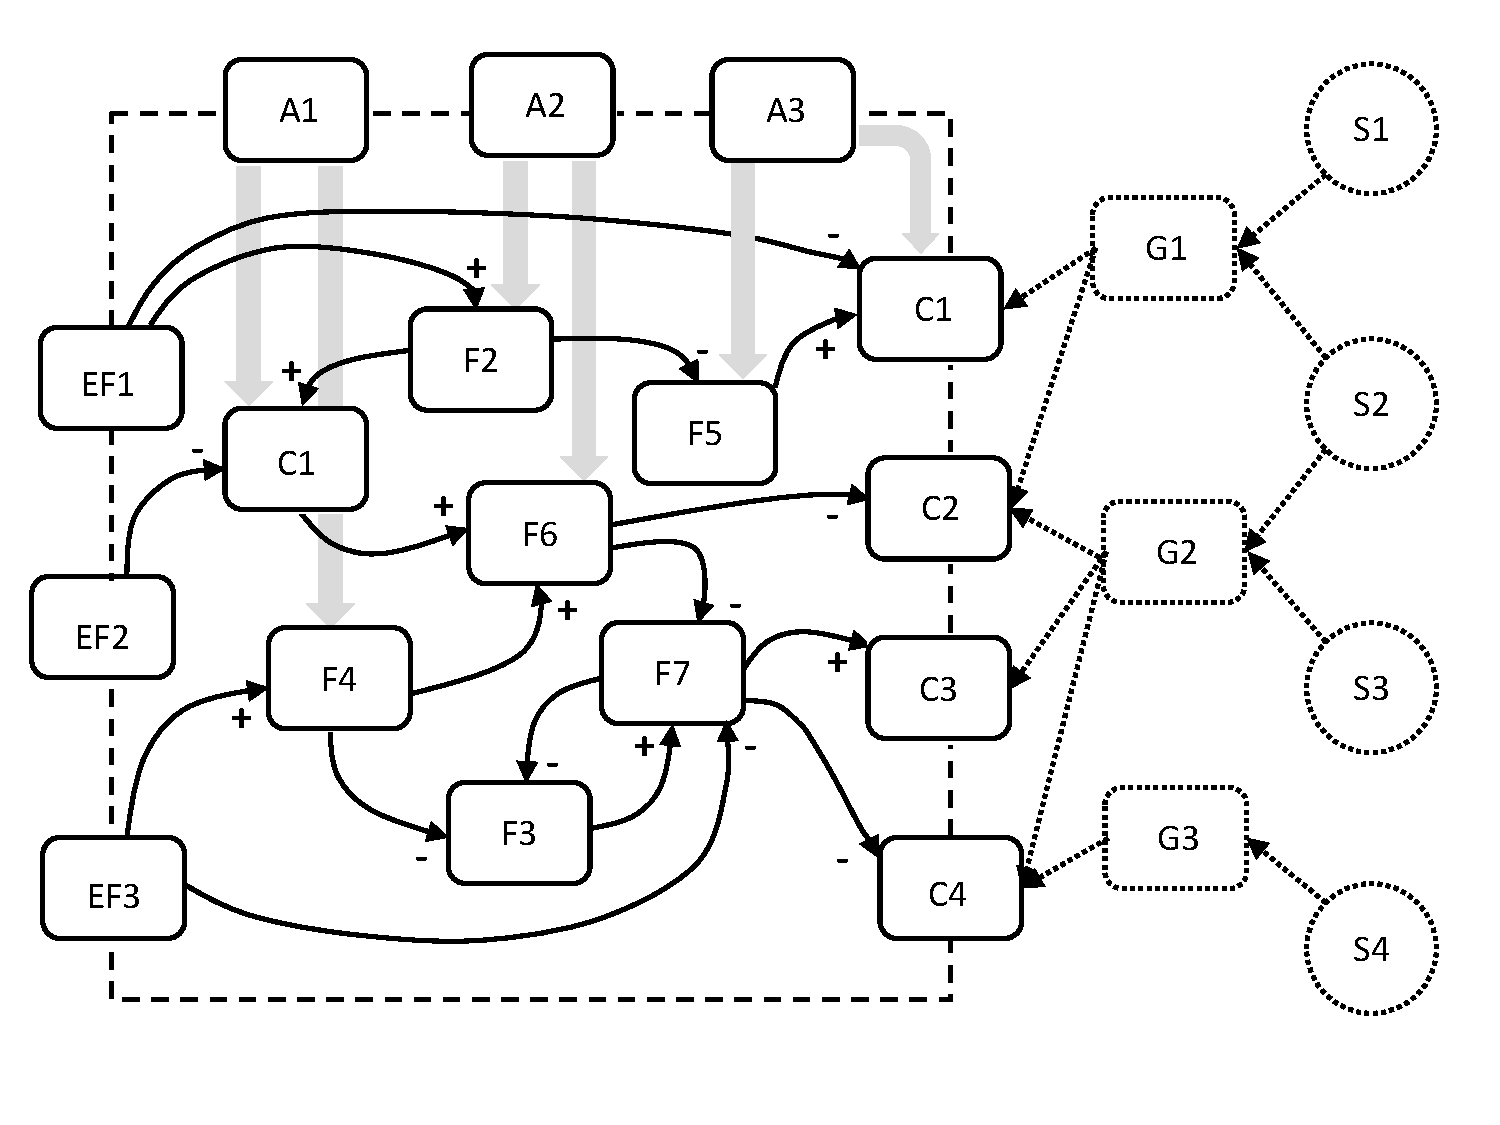
\includegraphics[width=0.9\textwidth]{../s4.pdf} }}%
%   \caption{The structure of a GRACeFUL concept map}%
%   \label{fig:cm}%
% \end{figure}

\section{GenericLibrary: a DSL for GCMs}

TODO: quote short parts of D4.1 and highlight similarities and differences
\todo{Make nicer}
GenericLibrary, henceforth abbreviated to GL, is a DSL for descriptions
of GRACeFUL concept map components embedded in the Haskell programming language.
The DSL addresses the issue of bridging the gap between constraint programming
and the visualisation layer by providing abstractions for modular constraint programming.
These abstractions are targeted at simplifying the description of GRACeFUL concept maps.

The DSL is divided in to two parts. The first part, \texttt{GCM} \todo{GCM is a monad},
allows the user to describe the interactions of GRACeFUL concept map components
and has facilities for constructing new components from existing ones \todo{Also known as monadic bind}. The second part,
\texttt{CP} \todo{CP is also a monad}, features primitives for constructing constraint programs
which describe the behaviour of an individual components.

\todo{How do we describe the available language constructs?}

\subsection{The language}\todo{Something about Haskell metaprogramming}
\todo{flesh out?}
As noted earlier, the GL language is primarily constructed from two different languages,
GCM and CP.

\todo{Something about how to include a CP component in a GCM one?}
\todo{\texttt{component :: CP a -> GCM ()}, the \texttt{GCM ()} type ensures nothing directly escapes from the scope of \texttt{CP} to \texttt{GCM}}
The GCM language supports constructing interfaces between components,
and has support for connecting the interface of different components.
The core abstraction in GL is that of the \texttt{Port}, a port is an
entity which represents the way two components interact. A component
exposes some information about the system, a pump may present one port
representing the amount of water being pumped through the pump and another
port representing the maximum flow the pump is able to produce. Ports
may be connected to each other through the \texttt{link} function.
\todo{something about the way in which relationships between factors are represented, i.e. \texttt{linkBy}}

The CP language supports reasoning about integer and floating-point arithmetic, boolean expressions,
and arrays. It has constructions like \texttt{createLVar} and \texttt{assert} for reasoning about
the internal behaviour of a GRACeFUL concept map component.

As can be seen there is a clear separation of concerns in GL between the high-level primitives
for constructing complicated components from simpler ones, represented in GCM, and the low level
implementation details with which the CP language is concerned.

\subsection{Expressing GRACeFUL concept map elements in GL}\todo{Relate to d4.1}
Many of the elements of GRACeFUL concept maps identified in \cite{D4.1} can be modeled in
GL using language primitives such as \texttt{linkBy} (for connections),
\texttt{createAction} (for actions), \texttt{assert} (for constraints) etc.
GL being an \textit{embedded} domain specific language featuring a rich set of primitive
operations for reasoning in the target domain allows the programmer to construct
abstractions which capture behaviour which generalises many of the concepts described
in \cite{D4.1}.


% Let us start with concepts and factors, which are, in a sense, the
% simplest elements of the GRACeFUL concept maps. Concepts are high-level
% descriptions of the components of a system, and they are refined into
% factors, which, as we have seen, determine the state of the system. The
% most important feature of a factor is that it is \emph{measurable}: it
% can take one value from a set of values. These values must be ordered,
% otherwise we do not have a notion of increasing or decreasing, as
% required by the use of factors in causal loop diagrams.
%
% Different factors can be associated with the same type of value. For
% example, there might be factors that represent temperatures in different
% parts of the system, such as ``water temperature'' and ``air
% temperature''. Even if the values of water temperature and air
% temperature happen to be equal, the two factors are still different.
% That means that a defining component of a factor is its identifier, its
% name. This suggests formalising the notion of a factor as a pair
% consisting of a name and a value. Such a formalisation makes explicit
% the part that stays the same, the name, in addition to the part that
% changes, the value. This is a common way of modelling states in
% functional programming.
%
% On the other hand, we can certainly create a causal loop diagram
% without knowing the value associated to the factors. None of the
% factors in the causal loops in Figures \ref{fig:cl1} and \ref{fig:cl2}
% have values associated with them. Therefore, we must formalise factors
% as pairs consisting of a name and \emph{potentially} of a value of an
% ordered type:
%
% \begin{Shaded}
% \begin{Highlighting}[]
% \KeywordTok{data} \NormalTok{(}\DataTypeTok{Ord} \NormalTok{value) }\OtherTok{=>} \DataTypeTok{Factor} \NormalTok{value  }\FunctionTok{=}  \DataTypeTok{MkFactor} \DataTypeTok{Name} \NormalTok{(}\DataTypeTok{Maybe} \NormalTok{value)}
% \end{Highlighting}
% \end{Shaded}
%
% For the moment, we can take the names of factors to be just strings:
%
% \begin{Shaded}
% \begin{Highlighting}[]
% \KeywordTok{type} \DataTypeTok{Name}  \FunctionTok{=}  \DataTypeTok{String}
% \end{Highlighting}
% \end{Shaded}
%
% Since we aim for a system based on qualitative reasoning, most of the
% types of value we shall use are going to be finite types, consisting of
% an enumeration of the symbols for possible landmark values and for the
% intervals delimited by the landmark values. For example, a very common
% type of qualitative values is:
%
% \begin{Shaded}
% \begin{Highlighting}[]
% \KeywordTok{data} \DataTypeTok{QualitativeValue}        \FunctionTok{=}  \DataTypeTok{Negative} \FunctionTok{|} \DataTypeTok{Zero} \FunctionTok{|} \DataTypeTok{Positive}
%                                 \KeywordTok{deriving} \NormalTok{(}\DataTypeTok{Eq}\NormalTok{, }\DataTypeTok{Ord}\NormalTok{)}
% \end{Highlighting}
% \end{Shaded}
%
% Here we have one landmark value, \VERB|\DecValTok{0}|, denoted by
% \VERB|\DataTypeTok{Zero}|, and two intervals:
% \VERB|\NormalTok{(}\FunctionTok{-}\NormalTok{inf, }\DecValTok{0}\NormalTok{)}|,
% denoted \VERB|\DataTypeTok{Negative}|, and
% \VERB|\NormalTok{(}\DecValTok{0}\NormalTok{, inf)}|, denoted
% \VERB|\DataTypeTok{Positive}|.
%
% Continuing the example of temperature factors above, we can have:
%
% \begin{Shaded}
% \begin{Highlighting}[]
% \NormalTok{t1, t2}\OtherTok{                 ::}  \DataTypeTok{Factor} \DataTypeTok{QualitativeValue}
% \NormalTok{t1                      }\FunctionTok{=}  \DataTypeTok{MkFactor} \StringTok{"Water Temperature"} \DataTypeTok{Nothing}
% \NormalTok{t2                      }\FunctionTok{=}  \DataTypeTok{MkFactor} \StringTok{"Air Temperature"} \NormalTok{(}\DataTypeTok{Just} \DataTypeTok{Positive}\NormalTok{)}
% \end{Highlighting}
% \end{Shaded}
%
% Here, \VERB|\NormalTok{t1}| represents the factor ``Water Temperature'',
% which does not currently have a defined value, and \VERB|\NormalTok{t2}|
% represents the factor ``Air Temperature'', whose current value is
% \VERB|\DataTypeTok{Positive}|.
%
% Factors are introduced via the refinement of \emph{concepts}. However,
% once the factors have been defined, concepts play no further role: in
% fact, they do not even appear in the current versions of the GRACeFUL
% concept maps. This is not surprising: concepts are high-level
% descriptions of parts of systems. In mathematical systems theory, (parts
% of) systems are \emph{defined} by their states, and so concepts are
% defined by the factors that they are ``refined'' into in the course of
% stakeholder interactions. Moreover, it is not clear that it is useful to
% distinguish between two concepts that are refined in identical sets of
% factors. Still, at this stage we think it useful to keep a record of the
% concept name, for example for the purpose of looking it up in a database
% of pre-defined (or pre-refined) concepts (thus creating re-usable
% building blocks). Formally, we have:
%
% \begin{Shaded}
% \begin{Highlighting}[]
% \KeywordTok{data} \DataTypeTok{Concept} \NormalTok{value        }\FunctionTok{=}  \DataTypeTok{MkConcept} \DataTypeTok{Name} \NormalTok{[}\DataTypeTok{Factor} \NormalTok{value]}
% \end{Highlighting}
% \end{Shaded}
%
% For simplicity, we have assumed that all the factors defining a concept
% have the same sets of possible values, in order to overcome some
% limitations of our Haskell notation.
%
% We now move on to the formalisation of goals and criteria. Criteria are
% similar to factors: they are part of the causal loop diagrams, hence
% have values in an ordered set, names, and maybe a definite value.
% Additionally, however, criteria are associated to \emph{predicates},
% which tell us whether a given value satisfies a concrete criterion or
% not:
%
% \begin{Shaded}
% \begin{Highlighting}[]
% \KeywordTok{type} \DataTypeTok{Predicate} \NormalTok{a    }\FunctionTok{=}  \NormalTok{(a }\OtherTok{->} \DataTypeTok{Bool}\NormalTok{)}
% \end{Highlighting}
% \end{Shaded}
%
% Therefore, we can formalise criteria as
%
% \begin{Shaded}
% \begin{Highlighting}[]
% \KeywordTok{data}  \NormalTok{(}\DataTypeTok{Ord} \NormalTok{value) }\OtherTok{=>} \DataTypeTok{Criterion} \NormalTok{value  }\FunctionTok{=}
%       \DataTypeTok{MkCriterion} \DataTypeTok{Name} \NormalTok{(}\DataTypeTok{Maybe} \NormalTok{value) (}\DataTypeTok{Predicate} \NormalTok{value)}
% \end{Highlighting}
% \end{Shaded}
%
% (Alternatively, we could have extended the type
% \VERB|\DataTypeTok{Factor} \NormalTok{value}|.)
%
% For example:
%
% \begin{Shaded}
% \begin{Highlighting}[]
% profit                  \OtherTok{::}  \DataTypeTok{Criterion} \DataTypeTok{QualitativeValue}
% \NormalTok{profit                   }\FunctionTok{=}  \DataTypeTok{MkCriterion} \StringTok{"Profit"} \NormalTok{(}\DataTypeTok{Just} \DataTypeTok{Zero}\NormalTok{) isPositive}
%                             \KeywordTok{where}
%                             \NormalTok{isPositive x }\FunctionTok{=} \NormalTok{x }\FunctionTok{>} \DataTypeTok{Zero}
% \end{Highlighting}
% \end{Shaded}
%
% introduces a criterion formalising ``profits should be (strictly)
% positive'', where the current value, \VERB|\DataTypeTok{Zero}|, does not
% satisfy the criterion.
%
% Criteria result from the refinement of goals, just as factors result
% from the refinement of concepts. It is no surprise, therefore, that the
% formalisation of goals will be just like that of concepts:
%
% \begin{Shaded}
% \begin{Highlighting}[]
% \KeywordTok{data} \DataTypeTok{Goal} \NormalTok{value        }\FunctionTok{=}  \DataTypeTok{MkGoal} \DataTypeTok{Name} \NormalTok{[}\DataTypeTok{Criterion} \NormalTok{value]}
% \end{Highlighting}
% \end{Shaded}
%
% At this point, it is useful to briefly discuss an essential difference
% between \emph{formalisation} and \emph{implementation}. The
% implementation of goals in the GRACeFUL system will very likely be much
% more complex than the formalisation presented here. We mentioned the
% possibility of looking up goals in a library of pre-defined goals, in
% order to assist the stakeholders in their search for adequate criteria.
% We might have various kinds of pre-defined goals, which might themselves
% be related in complicated ways, for example in order to assess
% inconsistencies between them. We could use \emph{ontologies} for the
% representation of goals, (and, for that matter, also concepts, factors,
% criteria, etc.), linking to Haskell RDF libraries, etc. Therefore, the
% implementation of \VERB|\DataTypeTok{Goal}| will likely result in a more
% complex datatype, such as:
%
% \begin{Shaded}
% \begin{Highlighting}[]
% \KeywordTok{data} \DataTypeTok{Goal}            \FunctionTok{=}  \DataTypeTok{GoalRDF} \DataTypeTok{Triple}
%                      \FunctionTok{|}  \DataTypeTok{G1} \DataTypeTok{PreDefinedG1}
%                      \FunctionTok{|}  \DataTypeTok{G2} \DataTypeTok{PreDefinedG2}
%                      \FunctionTok{|}  \FunctionTok{...}
%                      \FunctionTok{|}  \DataTypeTok{FreeFormGoal} \DataTypeTok{String}
% \end{Highlighting}
% \end{Shaded}
%
% Here, we are only concerned with \emph{understanding} as clearly as
% possible the notion of goal, factor, etc. as pertaining to their use in
% the GRACeFUL concept maps. We do not search for the most efficient
% representation in computational terms. We are also stripping away
% anything that does not belong to the essence of these notions \emph{as
% used in the concept maps}. One reason for this is that the formalisation
% undertaken here will be part of the \emph{specifications} to the
% implementations carried out in the course of the project. The simpler
% the specification, the likelier it is that it will be correctly
% understood and implemented. Moreover, since the specification is that
% against which we measure the correctness of the implementation, it is
% important that we do not overly constrain this implementation, for
% example by deciding that goals are going to be represented via RDF
% triples. At this stage, such a decision would be largely arbitrary.
%
% Now that we have formalised factors and criteria, the nodes of the
% causal loop diagrams, we can formalise these diagrams themselves. As
% mentioned above, these are instances of simple, directed graphs with
% labelled connections. The following datatype represents a simple
% directed graph, parametrised on the types of nodes and connections:
%
% \begin{Shaded}
% \begin{Highlighting}[]
% \KeywordTok{data} \DataTypeTok{Graph} \NormalTok{node conn  }\FunctionTok{=}  \DataTypeTok{MkGraph} \NormalTok{((node, node) }\OtherTok{->} \DataTypeTok{Maybe} \NormalTok{conn)}
% \end{Highlighting}
% \end{Shaded}
%
% In (other) words, a graph is given by a function which, to every ordered
% pair of nodes (a source and a target), associates either no connection,
% or just one connection.
%
% The connections in a causal loop diagram are labelled either with a
% plus, or a minus:
%
% \begin{Shaded}
% \begin{Highlighting}[]
% \KeywordTok{data} \DataTypeTok{Connection}       \FunctionTok{=}  \DataTypeTok{Plus} \FunctionTok{|} \DataTypeTok{Minus}
% \end{Highlighting}
% \end{Shaded}
%
% The nodes of our causal loop diagrams are either factors or criteria:
%
% \begin{Shaded}
% \begin{Highlighting}[]
% \KeywordTok{type} \DataTypeTok{Node} \NormalTok{value       }\FunctionTok{=}  \DataTypeTok{Either} \NormalTok{(}\DataTypeTok{Criterion} \NormalTok{value) (}\DataTypeTok{Factor} \NormalTok{value)}
% \end{Highlighting}
% \end{Shaded}
%
% Therefore, we can formalise a causal loop as
%
% \begin{Shaded}
% \begin{Highlighting}[]
% \KeywordTok{type} \DataTypeTok{CausalLoop} \NormalTok{value  }\FunctionTok{=}  \DataTypeTok{Graph} \NormalTok{(}\DataTypeTok{Node} \NormalTok{value) }\DataTypeTok{Connection}
% \end{Highlighting}
% \end{Shaded}
%
% GRACeFUL concept maps represent an enrichment of the causal loops with
% nodes representing the possible (atomic) actions and with nodes and
% links representing constraints between actions and factors.
%
% Actions can influence the nodes of a causal loop diagram, by changing
% the value associated with that node. We can formalise such an influence
% as a function that can return a new value for a given node (or
% \VERB|\DataTypeTok{Nothing}| in the case of ``no influence'').
%
% \begin{Shaded}
% \begin{Highlighting}[]
% \KeywordTok{type} \DataTypeTok{Influence} \NormalTok{value  }\FunctionTok{=}  \DataTypeTok{Node} \NormalTok{value }\OtherTok{->} \DataTypeTok{Maybe} \NormalTok{value}
% \end{Highlighting}
% \end{Shaded}
%
% An action is then defined as a named influence:
%
% \begin{Shaded}
% \begin{Highlighting}[]
% \KeywordTok{data} \DataTypeTok{Action} \NormalTok{value     }\FunctionTok{=}  \DataTypeTok{MkAction} \DataTypeTok{Name} \NormalTok{(}\DataTypeTok{Influence} \NormalTok{value)}
% \end{Highlighting}
% \end{Shaded}
%
% An alternative policy is, similar to a goal or a concept, a named set of
% actions:
%
% \begin{Shaded}
% \begin{Highlighting}[]
% \KeywordTok{data} \DataTypeTok{Alternative}  \NormalTok{value    }\FunctionTok{=}  \DataTypeTok{MkAlternative} \DataTypeTok{Name} \NormalTok{[}\DataTypeTok{Action} \NormalTok{value]}
% \end{Highlighting}
% \end{Shaded}
%
% One of the major outputs of the GRACeFUL system will be a list of
% alternatives which meet the goals and the constraints; we could define
%
% \begin{Shaded}
% \begin{Highlighting}[]
% \KeywordTok{type} \DataTypeTok{GRACeFUL_Solution} \NormalTok{value  }\FunctionTok{=}  \NormalTok{[}\DataTypeTok{Alternative} \NormalTok{value]}
% \end{Highlighting}
% \end{Shaded}
%
% As we have seen in the previous section, actions can be constrained by
% factors (e.g., investments are constrained by the available capital).
% This is common in systems theory, where the set of controls that can be
% used when the system is in a given state depend on that state.
%
% Similarly, there can be constraint relations between the factors
% themselves. These constraints can either be associated with concepts, as
% in the case in which the constraints relate factors stemming from the
% refinement of the same concept, or with interactions between concepts.
%
% The constraint relations are, in general, non-causal, and are thus
% genuine enhancements over a causal loop diagram. They can sometimes be
% represented by directed links, for example, ``source value may not
% exceed target value'', but in general they will require the introduction
% of a new kind of node. It is easy to see that a constraint such as
% ``only one of these three factors may be negative'' is not expressible
% as a link between two factors.
%
% Constraints that can be expressed as links can be formalised as
%
% \begin{Shaded}
% \begin{Highlighting}[]
% \KeywordTok{data} \DataTypeTok{ConstraintLink} \NormalTok{value  }\FunctionTok{=}  \DataTypeTok{MkConstraintLink} \NormalTok{(}\DataTypeTok{Predicate} \NormalTok{(value, value))}
% \end{Highlighting}
% \end{Shaded}
%
% This corresponds to the intuition that we can model a constraint as a
% link only if it is a binary relation.
%
% For example:
%
% \begin{Shaded}
% \begin{Highlighting}[]
% doesNotExceed             \OtherTok{::}  \DataTypeTok{Ord} \NormalTok{value }\OtherTok{=>} \DataTypeTok{ConstraintLink} \NormalTok{value}
% \NormalTok{doesNotExceed              }\FunctionTok{=}  \DataTypeTok{MkConstraintLink} \NormalTok{gt}
%                               \KeywordTok{where}
%                               \NormalTok{gt (v1, v2) }\FunctionTok{=} \NormalTok{v1 }\FunctionTok{<=} \NormalTok{v2}
% \end{Highlighting}
% \end{Shaded}
%
% Constraints between more than two factors cannot be modelled as links.
% For these, we need to introduce nodes which collect the values of
% several factors or actions, and check if these values satisfy the
% constraint, operating in a similar way to the criteria. As opposed to
% the criteria, the value associated to a constraint is either true, or
% false.
%
% In a binary relation such as \VERB|\NormalTok{doesNotExceed}|, we can
% distinguish between the two elements (``what does not exceed what?'')
% based on the source and target order of a directed link. This is not
% possible in the case of a constraint represented by a node. Therefore,
% the various roles of the related values must be indicated by the links.
% As an example, consider the constraint given by
%
% \begin{Shaded}
% \begin{Highlighting}[]
% inBetweenPred             \OtherTok{::}  \DataTypeTok{Ord} \NormalTok{value }\OtherTok{=>} \DataTypeTok{Predicate} \NormalTok{(value, value, value)}
% \NormalTok{inBetweenPred (v1, v2, v3) }\FunctionTok{=}  \NormalTok{v1 }\FunctionTok{<=} \NormalTok{v2 }\FunctionTok{&&} \NormalTok{v2 }\FunctionTok{<=} \NormalTok{v3}
% \end{Highlighting}
% \end{Shaded}
%
% This constraint will be represented by a node. There will be three links
% into this node, representing the three arguments. These links will need
% to be labelled, in order for the constraint node to be able to tell
% which one of the arguments is associated to each link. We can introduce
% a type for these labels:
%
% \begin{Shaded}
% \begin{Highlighting}[]
% \KeywordTok{data} \DataTypeTok{Role}                  \FunctionTok{=}  \DataTypeTok{V1} \FunctionTok{|} \DataTypeTok{V2} \FunctionTok{|} \DataTypeTok{V3}
%                               \KeywordTok{deriving} \DataTypeTok{Eq}
% \end{Highlighting}
% \end{Shaded}
%
% A role link will connect nodes to a constraint node, specifying their
% role:
%
% \begin{Shaded}
% \begin{Highlighting}[]
% \KeywordTok{data} \DataTypeTok{RoleLink} \NormalTok{role         }\FunctionTok{=}  \DataTypeTok{MkRoleLink} \NormalTok{role}
% \end{Highlighting}
% \end{Shaded}
%
% Finally, a constraint node will be represented by a predicate on a list
% of role-value pairs:
%
% \begin{Shaded}
% \begin{Highlighting}[]
% \KeywordTok{data} \DataTypeTok{ConstraintNode} \NormalTok{role val  }\FunctionTok{=}  \DataTypeTok{MkConstraintNode} \NormalTok{(}\DataTypeTok{Predicate} \NormalTok{[(role, val)])}
% \end{Highlighting}
% \end{Shaded}
%
% For example, we can define the node associated to the
% \VERB|\NormalTok{inBetweenPred}| above by
%
% \begin{Shaded}
% \begin{Highlighting}[]
% inBetweenC                \OtherTok{::}  \DataTypeTok{Ord} \NormalTok{value }\OtherTok{=>} \DataTypeTok{ConstraintNode} \DataTypeTok{Role} \NormalTok{value}
% \NormalTok{inBetweenC                 }\FunctionTok{=}  \DataTypeTok{MkConstraintNode} \NormalTok{p}
%                               \KeywordTok{where}
%                               \NormalTok{p as }\FunctionTok{=} \NormalTok{inBetweenPred (toTriple as)}
% \end{Highlighting}
% \end{Shaded}
%
% (we omit the implementation of \VERB|\NormalTok{toTriple}|).
%
% There is one remaining element of the GRACeFUL concept map as presented
% above, namely the nodes representing the stakeholders. These are meant
% to relate the stakeholders to their goals, thus we can formalise them
% as:
%
% \begin{Shaded}
% \begin{Highlighting}[]
% \KeywordTok{data} \DataTypeTok{Stakeholder} \NormalTok{value  }\FunctionTok{=}  \DataTypeTok{MkStakeholder} \DataTypeTok{Name} \NormalTok{[}\DataTypeTok{Goal} \NormalTok{value]}
% \end{Highlighting}
% \end{Shaded}
%
% The nodes of the GRACeFUL concept maps are therefore:
%
% \begin{Shaded}
% \begin{Highlighting}[]
% \KeywordTok{data} \DataTypeTok{ConceptMapNode} \NormalTok{role value  }\FunctionTok{=}  \DataTypeTok{CN} \NormalTok{(}\DataTypeTok{Node} \NormalTok{value)}
%                                 \FunctionTok{|}  \DataTypeTok{AN} \NormalTok{(}\DataTypeTok{Action} \NormalTok{value)}
%                                 \FunctionTok{|}  \DataTypeTok{GN} \NormalTok{(}\DataTypeTok{Goal} \NormalTok{value)}
%                                 \FunctionTok{|}  \DataTypeTok{CO} \NormalTok{(}\DataTypeTok{ConstraintNode} \NormalTok{role value)}
%                                 \FunctionTok{|}  \DataTypeTok{SN} \NormalTok{(}\DataTypeTok{Stakeholder} \NormalTok{value)}
% \end{Highlighting}
% \end{Shaded}
%
% Besides the causal connections in the causal loop diagram, we also have
% links from actions to the factors and criteria they influence, from the
% criteria to the goals they assess, from stakeholders to the goals they
% ``own'', constraint links, and role links.
%
% \begin{Shaded}
% \begin{Highlighting}[]
% \KeywordTok{data} \DataTypeTok{ConceptMapConnection} \NormalTok{role value  }\FunctionTok{=}  \DataTypeTok{CC} \DataTypeTok{Connection}
%                                       \FunctionTok{|}  \DataTypeTok{ActionToNode}
%                                       \FunctionTok{|}  \DataTypeTok{CriterionToGoal}
%                                       \FunctionTok{|}  \DataTypeTok{CL} \NormalTok{(}\DataTypeTok{ConstraintLink} \NormalTok{value)}
%                                       \FunctionTok{|}  \DataTypeTok{RL} \NormalTok{(}\DataTypeTok{RoleLink} \NormalTok{role)}
%                                       \FunctionTok{|}  \DataTypeTok{StakeholderToGoal}
% \end{Highlighting}
% \end{Shaded}
%
% We can now define the GRACeFUL concept map as a simple, directed graph:
%
% \begin{Shaded}
% \begin{Highlighting}[]
% \KeywordTok{type} \DataTypeTok{ConceptMap} \NormalTok{role value  }\FunctionTok{=}  \DataTypeTok{Graph} \NormalTok{(}\DataTypeTok{ConceptMapNode} \NormalTok{role value)}
%                                      \NormalTok{(}\DataTypeTok{ConceptMapConnection} \NormalTok{role value)}
% \end{Highlighting}
% \end{Shaded}
%
% A concept map
% \VERB|\NormalTok{cm }\FunctionTok{=} \DataTypeTok{MkGraph} \NormalTok{f}|
% is \emph{valid} if:
%
% \begin{itemize}
% \item
%   \VERB|\NormalTok{f (cn1, cn2) }\FunctionTok{=} \DataTypeTok{ActionToNode}|
%   iff \VERB|\NormalTok{cn1}| is of the form
%   \VERB|\DataTypeTok{AN} \NormalTok{(}\DataTypeTok{MkAction} \NormalTok{name infl)}|,
%   \VERB|\NormalTok{cn2}| is of the form
%   \VERB|\DataTypeTok{CN} \NormalTok{node}|, and
%   \VERB|\NormalTok{infl node}| is not \VERB|\DataTypeTok{Nothing}|.
% \item
%   \VERB|\NormalTok{f (cn1, cn2) }\FunctionTok{=} \DataTypeTok{CriterionToGoal}|
%   iff \VERB|\NormalTok{cn1}| is of the form
%   \VERB|\DataTypeTok{CN} \NormalTok{(}\DataTypeTok{Left} \NormalTok{crit)}|,
%   \VERB|\NormalTok{c2}| is of the form
%   \VERB|\DataTypeTok{GN} \NormalTok{(}\DataTypeTok{MkGoal} \NormalTok{name crits)}|,
%   and \VERB|\NormalTok{crit}| is an element of \VERB|\NormalTok{crits}|.
% \item
%   \VERB|\NormalTok{f (cn1, cn2) }\FunctionTok{=} \DataTypeTok{StakeholderToGoal}|
%   iff \VERB|\NormalTok{cn1}| is of the form
%   \VERB|\DataTypeTok{SN} \NormalTok{(}\DataTypeTok{MkStakeholder} \NormalTok{sname goals)}|,
%   \VERB|\NormalTok{cn2}| is of the form
%   \VERB|\DataTypeTok{GN} \NormalTok{goal}|, and \VERB|\NormalTok{goal}|
%   is an element of \VERB|\NormalTok{goals}|.
% \item
%   \VERB|\NormalTok{f (cn1, cn2) }\FunctionTok{=} \DataTypeTok{CC} \NormalTok{plusOrMinus}|
%   only if \VERB|\NormalTok{cn1}| is of the form
%   \VERB|\DataTypeTok{CN} \NormalTok{node1}| and \VERB|\NormalTok{cn2}|
%   is of the form \VERB|\DataTypeTok{CN} \NormalTok{node2}|.
% \item
%   \VERB|\NormalTok{f (cn1, cn2) }\FunctionTok{=} \DataTypeTok{RL} \NormalTok{r}|
%   only if \VERB|\NormalTok{cn1}| is a factor node or an action node, and
%   \VERB|\NormalTok{cn2}| is a constraint node.
% \item
%   \VERB|\NormalTok{f (cn1, cn2) }\FunctionTok{=} \DataTypeTok{CL} \NormalTok{cl}|
%   only if \VERB|\NormalTok{cn1}| and \VERB|\NormalTok{cn2}| are factors
%   or actions.
% \end{itemize}

\subsection{Example: Runoff flow}\label{example-runoff-flow}

\todo{Insert figure showing a graphical view?}

\subsection{Example: Runoff flow: DSL textual
input}\label{example-runoff-flow-dsl-textual-input}

\todo{Say something about more the collection of examples available online: }
The collection of examples is available in the \verb+examples/+ directory of the GitHub repository \href{https://github.com/GRACeFUL-project/GenericLibrary}{GenericLibrary}:

% -- A GCM representing a simluation of the swedish energy system
% energySystem :: GCM ()
% SmallExample.hs

\subsection{Example: Runoff flow}
\label{example-runoff-flow}

We show a small GL program which models a rain runoff area, like a
town square, which has been provided with a pump to alleviate possible
flooding issues (this is a common procedure in countries like the
Netherlands).
%
This example is a small part of a larger model used in the CRUD case
study meant to show how GL can be employed to model concrete problems
in CRUD.


\subsubsection{DSL textual input}
\label{example-runoff-flow-dsl-textual-input}

\todo{some explaining text?}

\begin{verbatim}
pump :: Float -> GCM (Port Float, Port Float)
pump ... -- As before

rain :: Float -> GCM (Port Float)
rain ... -- As before

storage :: Float -> GCM (Port Float, Port Float, Port Float)
storage cap = do
  inflow   <- createPort
  outlet   <- createPort
  overflow <- createPort
  component $ do
    currentStored <- createVariable
    inf <- value inflow
    out <- value outlet
    ovf <- value overflow
    sto <- value currentStored
    assert $ sto === inf - out - ovf
    assert $ sto `inRange` (0, lit cap)
    assert $ (ovf .> 0) ==> (sto === lit cap)
    assert $ ovf .>= 0
  return (inflow, outlet, overflow)

example :: GCM ()
example = do
  (inflowP, outflowP) <- pump 5
  (inflowS, outletS, overflowS) <- storage 4
  rainflow <- rain 10

  link inflowP outletS
  link inflowS rainflow

  output "Overflow" overflowS
\end{verbatim}

When we run the above program we get the output

\begin{verbatim}
ghci> runGCM example
{"Overflow" : 0}
\end{verbatim}
\todo{More explanation needed!}

\todo{Say something about actions!}

\subsection{Software infrastructure (around the
DSL)}\label{software-infrastructure-around-the-dsl}

\todo{Replace by a more current description of the software status}

\todo{Should we even describe the two different software stacks}

\begin{itemize}
\item
  (VIS layer)
\item
  GenericLibrary
\item
  (MiniZinc)
\item
  (VIS layer)
\item
  GraphDSL (describe the graph) + ConstraintDSL (still ongoing work)
\item
  QPNModeler: encodes the Qualitative Probabilistic Network semantics
\item
  haskelzinc: Haskell interface to (and from) MiniZinc
\item
  (MiniZinc)
\end{itemize}

\section{Installation and software requirements}
\label{install-script-and-requirements}

%% -- Installation instructions -----------------------------------------------
%% ----------------------------------------------------------------------------

The purpose of this section is to outline the process of installing
the GRACe software and its require dependencies.
%
Section~\ref{install-overview} provides an overview of the software
dependencies required for development using GRACe.
%
Section~\ref{install-docker} provides installation instructions for a
platform-independent package utilising the
\href{https://www.docker.com/}{Docker}
platform.

%% -- Software dependencies ---------------------------------------------------

\subsection{Software dependencies}
\label{install-overview}

The GRACe language is implemented in
\href{https://www.haskell.org/}{Haskell} and uses the solver tools
from the \href{http://www.minizinc.org/}{MiniZinc} software
distribution.
%
Specifically, development and execution of GRACe programs requires the
following software dependencies to be met:

\begin{itemize}
\item The MiniZinc and Gecode solver software.
%
  These can be found in the MiniZinc software bundle.
%
\item A complete Haskell toolchain able to download packages from
  \href{https://hackage.haskell.org/}{Hackage}.
%
  Two alternative tools (Stack and Cabal) are suitable for this
  purpose, and both are provided by
  \href{https://www.haskell.org/platform/}{the Haskell Platform}.
\end{itemize}

Instructions for installing and using these components are available
in the {GRACe} repository on
\href{https://github.com/GRACeFUL-project/%
  GRACe/blob/master/doc/INSTALL.md}{GitHub}.
%
Alternatively, for those who only wish to run the GRACe
examples, we provide instructions in the following section.

%% -- Using Docker ------------------------------------------------------------

\subsection{Installation using Docker}
\label{install-docker}

Download and install the Docker app from \url{https://www.docker.com/products/docker}.
%
Open a terminal (or the \emph{command prompt} under Windows) and
execute
\begin{verbatim}
  docker pull eugraceful/generic-library
  docker run --rm eugraceful/generic-library
\end{verbatim}

This will download and execute the example located at
\href{https://github.com/GRACeFUL-project/GRACe/blob/master/examples/Examples.hs}{examples/Examples.hs}.


\section{Semantics}\label{semantics}
\todo{Add something about semantics of GenericLibrary?}
\todo{Flesh out this section/transition, refer to D4.1 (or section above describing
  differences from D4.1)}
Originally our main focus was writing a DSL to describe causal loop diagrams (CLDs) and
translate them to system dynamics models, and we spent some time considering
formal semantics that could aid in reasoning about CLDs.

We have modelled CLDs within the \verb|GenericLibrary|, the code for this model
can be seen in the file \verb|QualitativeExample.hs|. \\

\subsection{Causal loop diagrams}

A causal loop diagram (CLD) is a directed graph used to display causal
relationships between variables.
%
The vertices represent the variables and the edges represent qualitative
causal relationships, which can be positive or negative.

We would like to define a semantic that aids us in reasoning about CLDs and will
describe two such semantics here.

\paragraph{Notation}
We denote a positive causal relationship between $A$ and $B$ by
$A\xrightarrow{+} B$ and a negative one by $A \xrightarrow{-} B$.
%
Then $A \xrightarrow{+} B$ means that an increase in $A$ causes an
increase in $B$, while a decrease in $A$ causes a decrease in $B$.
%
On the other hand, $A\xrightarrow{-} B$ means that an increase in $A$
causes a decrease in $B$ (and conversely a decrease in $A$ causes an
increase in $B$).
%
We denote the sign of the edge from $A$ to $B$ by $s_{AB}$, so
$s_{AB}= +$ if $A\xrightarrow{+} B$ and $s_{AB}=-$ if
$A\xrightarrow{-} B$.

A vertex $A$ also has a sign $s_A$ that denotes the total influence on $A$, so
$s_A=+$ if there is an increase in $A$, $s_A=-$ if there is a decrease, $s_A=0$
if there is no change and $s_A=?$ if we cannot determine the change in $A$.

\subsection{QPN approach}

One approach to modelling and reasoning about CLDs is by using qualitative
probabilistic networks (QPNs).

A QPN is defined as a directed
acyclic graph $G=(V,E)$ where the vertices, $V$, correspond to
variables and the edges, $E$ to qualitative probabilistic influences.
%
These influences can be positive (+) or negative (-).
%
Later, when computing transitive influences we will also use (?) for
ambiguous and (0) for probabilistic independence

The meaning of signs on edges is defined according to first order
stochastic dominance, as follows:

Let $F_B(\cdot|a_i, x)$ be the cumulative distribution function (CDF) for
$B$ given $A=a_i$. Then $s_{AB}=+$ means that for all possible values
$a_1,a_2$ of $A$ where $a_1\geq a_2$, we must have:
\[F_B(b_0|a_1, x)\leq F_B(b_0|a_2, x),\]
that is,
\[P(B \leq b_0| A = a_1, x)\leq P(B\leq b_0| A = a_2, x)\]
for all possible values $b_0$ of $B$ and any consistent context $x$.
The context $x$ ranges over all possible assignments to the
variables other than $A$ that influence $B$, that are consistent with both
$A=a_1$ and $A=a_2$.
%
The definition of $s_{AB}=-$ is the same but with $a_1\leq a_2$.

In simpler terms, $s_{AB} = +$ means that greater values of $A$ mean
greater values of $B$ are more likely, and $s_{AB}=-$ means that
greater values of $A$ mean smaller values of $B$ are more likely.

These influences are symmetric, that is, if the edge from $X$ to $Y$ is reversed
we must have $s_{XY} = s_{YX}$.
%
Due to this symmetry it is possible to propagate an observed increase
or decrease of one variable around the graph and find whether other
variables are then likely to have increased or decreased.

TODO: cite Wellman etc.

This definition is broad enough to
apply to many different systems and
be applicable to various real world situations.

We found some issues with QPNs that lead us to explore other
approaches.
%
First of all, since QPNs were originally defined for acyclic graphs
and the theory on them relies on acyclicity, they may not be the best
fit to describe CLDs, in which cycles (feedback loops) are an important
feature.
%
Inference on QPNs containing loops is difficult to implement and can
lead to ambiguous results.

Second, the formal semantics of inference on QPNs is difficult to
formalize since it relies heavily on not-so-simple probability theory.
%
(And stakeholder sessions will not produce data on probability
distributions.)

Additionally, as QPNs are defined solely based on qualitative
relationships there is no obvious way to expand them to also describe
quantitative relationships.

Lastly, since all inference in QPNs is probabilistic it leads to
results that may not be as meaningful or concrete as we would like,
such as ``there is a heightened probability that $x$ has increased'',
rather than ``$x$ has increased''.
%
For instance, a variable may decrease even though the cumulative
probabilistic influence on it is positive.

\subsubsection{Difference equation approach}

Inspired by a system of tanks with water flowing from one to another,
and in search of semantics that might also be extended to quantitative
reasoning, we came up with the following approach.

We consider the values of the graph's vertices to be functions of the same
variable, such as a time variable $t$.

If we have a graph with two vertices, $X$ and $Y$, and one edge from $X$
to $Y$, then $s_{XY}=+$ implies that
\[\frac{\partial Y}{\partial t} = G(X(t)),\]
where $G$ is a monotonically increasing function (monotonically decreasing for negative
causality, $s_{XY}=-$).

If the vertex $Y$ has multiple parent vertices $X_1,\ldots,X_n$, then
$\frac{\partial Y}{\partial t}$ depends on all the parent vertices. We can
isolate the effect of a single parent vertex
 $X$ on $Y$ by differentiation.

In general we can then describe the causal relationship from $X$ to
$Y$ as
\[\frac{\partial\left( \frac{\partial Y(t)}{\partial t} \right)}{\partial Y(t)} =
  g(X(t)),\]

where $g$ has a primitive function $G$ such that $G$ is monotonically
increasing if $s_{XY}=+$ and monotonically decreasing if $s_{XY}= -$.

This is somewhat more nuanced than $CLDs$ as they are described above,
where $s_{XY}=+$ implies that an increase in $X$ leads to an increase
in $Y$, and a decrease in $X$ to a decrease in $Y$.
%
Here we may have some threshold value $x_0$ for $X$, where $G(x_0) = 0$,
above which $X$ always causes an increase in $Y$, but an increase in $X$
causes a faster rate of increase in $Y$ and a decrease in $X$ causes a
slowed rate of increase in $Y$, and vice versa.

Note that though $G(X)$ is monotonically increasing, it may not be strictly
increasing, so we could for instance have $G(X) = 0$ for all $X < C$
for some threshold value $C$.

If the vertex $Y$ has parent vetices $X_1,\ldots,X_n$, then we have
\[\frac{\partial Y}{\partial t} = \sum_{i=1}G_i(X_i),\]
where $G_i$ is monotonically increasing if $s_{X_iY}=+$ but monotonically
decreasing if $s_{X_iY}=-$.

In a discrete time system we consider $\Delta(X_t) = X_t - X_{t-1}$
instead of $\frac{\partial X}{\partial t}$, and write
$\Delta(X_t) = G(Y_{t-1})$ instead of
$\frac{\partial X}{\partial t} = G(Y(t))$.
%
In simple cases we may only consider one time step with two values of
$t$, $t_{start}$ and $t_{end}$.

Here we explore how this approach relates to qualitative reasoning,
but it could be extended to quantitative reasoning by solving
appropriate differential equations.

\paragraph{Simple qualitative model}

We consider a qualitative discrete time system where all values of
vertex variables are either +, -, 0, or ? (where ? is an ambiguous value assigned
to a variable whose value cannot be deduced). These values have the partial
ordering $- < 0 < +$, but ? cannot be compared to the other values. In place of
addition and multiplication we have the operations $\oplus$ and $\otimes$, whose
behavior can be seen in the following tables:
\begin{center}
\begin{tabular}{c|cccc}
$\oplus$ & + & - & 0 & ?\\
\hline
  +   & +  & ? & + & ?\\
  -   & ?  & - & - & ?\\
  0   & +  & - & 0 & ?\\
  ?   & ?  & ? & ? & ?\\
\end{tabular}
\quad
\begin{tabular}{c|cccc}
$\otimes$ & + & - & 0 & ?\\
\hline
  +   & +  & - & 0 & ?\\
  -   & -  & + & 0 & ?\\
  0   & 0  & 0 & 0 & 0\\
  ?   & ?  & ? & 0 & ?\\
\end{tabular}
\end{center}
The only
strictly increasing function in this system is the identity function $id(x) =
x$, and the only strictly decreasing function is the negation function $neg(x) =-\otimes x$.

For simplicity we consider the case where all initial values are
set to zero and $G_e(0)=0$, for all edges $e$. We only consider edge functions
$G_e$ where $G_e(?) = ?$, since we shouldn't be able to make unambiguous
deductions based on ambiguous values.
%

This is convenient for qualitative reasoning since then we are only
concerned with increases and decreases rather than numerical values.
%
The value of variable $X$ at time $t$, which we denote by $X_t$, then tells us whether there has been a net
increase or decrease in $X$.

Consider a graph with three vertices, $Z$ and its two parents
$X$ and $Y$, $X\xrightarrow{s_{XZ}} Z$ and $Y\xrightarrow{s_{YZ}} Z$.
%
Then we have
\[\Delta(Z_t) = G_{XZ}(X_{t-1}) \oplus G_{YZ}(Y_{t-1}),\]
where $G_{XZ}$ and $G_{YZ}$ are monotonically increasing or decreasing in
accordance with $s_{XZ}$ and $s_{YZ}$.
%
If we only allow strictly increasing/decreasing functions we then have
\[\Delta(Z_t) = (s_{XZ}\otimes X_{t-1})\oplus (s_{YZ}\otimes Y_{t-1}).\]

Consider a graph with three vertices $A$, $B$ and $C$ and two edges,
$A\xrightarrow{s_{AB}} B$ and $B\xrightarrow{s_{BC}} C$. Then we have
\begin{align*}
\Delta(C_t) &= G_{BC}(B_{t-1})\\
&= G_{BC}(B_{t-2} \oplus \Delta(B_{t-1}))\\
&= G_{BC}(B_{t-2}  \oplus G_{AB}(A_{t-2}))\\
\end{align*}

If $G_{BC}$ is linear, as is the case when we restrict the available functions
to the strictly increasing/decreasing $id$ and $neg$,
we then have
\[\Delta(C_t) = G_{BC}(B_{t-2})\oplus G_{BC}\circ G_{AB}(A_{t-2}).\]

If we only allow strictly increasing/decreasing functions we then have
\[\Delta(C_t) = (s_{BC}\otimes B_{t-2})\oplus (s_{BC}\otimes s_{AB}\otimes A_{t-2}),\]

\end{document}
